\chapter{Liquid Dynamics}


The dynamics of a molecular system is characterised by two main elements, the diffusion of the particles through the liquid and the rotational motion of those particles. Understanding these properties of the liquid provide the basis for further study giving estimates of the timescales that events are likely to occur at. It also provides important information about the range of temperatures at which the particular system can be studied. The molecules that we have chosen for study are shown in \textfigref{my mols}, these molecules were chosen to be representative of the range of samples and also with the possibility of showing interesting behaviour as discussed in \textsecref{shapes of interest}. Through the rest of this thesis the molecules will be referred to by symbols as indicated in \textfigref{my mols}.

\begin{figure}
    \centering
    \begin{subfigure}{0.3\textwidth}
        \includegraphics[width=\linewidth]{{{Snowman-0.637556-1.637556}}}
        \caption{Snowman $r=0.637556,\,d=1.637556$ (\scon)}
        \label{fig:scon}
    \end{subfigure}
    \begin{subfigure}{0.3\textwidth}
        \includegraphics[width=\linewidth]{{{Snowman-0.637556-1.0}}}
        \caption{Snowman $r=0.637556,\,d=1.0$ (\sone)}
        \label{fig:sone}
    \end{subfigure}
    \begin{subfigure}{0.3\textwidth}
        \includegraphics[width=\linewidth]{{{Snowman-0.637556-1.0}}}
        \caption{Trimer $r=0.637556,\,d=1.0,\,\theta=120$ (\tri)}
        \label{fig:tri}
    \end{subfigure}
    \caption[Molecules chosen for further study]{The molecules chosen for study in this chapter. }
    \label{fig:my mols}
\end{figure}

\section{Dynamics of \sone}

\begin{figure}
    \begin{subfigure}{0.5\linewidth}
        \includegraphics[width=\textwidth]{{{Snowman-0.637556-1.0-msd}}}
        \caption{MSD}
        \label{fig:snowman 0.637556 1.0 msd}
    \end{subfigure}
    \begin{subfigure}{0.5\linewidth}
        \includegraphics[width=\textwidth]{{{Snowman-0.637556-1.0-r1}}}
        \caption{R1}
        \label{fig:snowman 0.637556 1.0 r1}
    \end{subfigure}
    \begin{subfigure}{0.5\textwidth}
        \includegraphics[width=\textwidth]{{{Snowman-0.637556-1.0-struct}}}
        \caption{structure function}
        \label{fig:snowman 0.637556 1.0 structure}
    \end{subfigure}
    \begin{subfigure}{0.5\textwidth}
        \includegraphics[width=\textwidth]{{{Snowman-0.637556-1.0-r2}}}
        \caption{r2}
        \label{fig:snowman 0.637556 1.0 r2}
    \end{subfigure}
    \caption{Snowman 0.637556 1.0}
    \label{fig:snowman 0.637556 1.0}
\end{figure}

The four plots in~\textfigref{snowman 0.637556 1.0} are the main features of each system. The MSD tells us about the translational motion of the molecules, how fast they move through space and the timescales required for them to enter a diffusive regime, moving out of the ballistic region. The rotational relaxations tell us about the timescales of rotations, these can be completely uncorrelated from the diffusion, molecules can rotate around a point with no diffusion, they can also diffuse in a straight line with no rotational motion. The final function, the structure function is a combination of the both rotation and diffusion, the structure function is a binary function
\begin{align}
    F(t) = \begin{cases}
        \quad0 &\text{if } \Delta \vect x > 0.3 \\
        \quad1 &\text{if } \Delta \vect x \leq 0.3
    \end{cases}
\end{align}
where $\Delta \vect x$ is the distance of each individual particle from the initial position. The combination of the rotation and diffusion is a result of considering each particle individually rather than as molecules. This approach is also more in line with what would be observed experimentally, x-ray diffraction sees areas of high electron density separately, the atoms, rather than molecules.

Along with being averaged over the ensemble these functions are averaged over many overlapping time points. This removes any large fluctuations since the initial configuration is a random configuration in the space of all possible configurations~\tocite. The simulation can be thought of as sampling all possible configurations, this is the premise of statistical thermodynamics, so any configuration sufficiently separated in time is another random configuration from which it is reasonable to start a new analysis.

All the properties so far have been investigating the bulk properties of the molecules, however in the highly supercooled region in which we are interested in, the dynamics of the system are often heterogeneous, there are spatially separated regions of highly mobile particles and regions of slow moving particles. \textfigref{snowman 0.637556 1.0 moved} shows that there are these dynamically heterogeneous areas in the snowman molecule. It is also important to note that there are also dynamically heterogeneous rotations, these are not something that have been studied before~\tocheck. At a most basic level these measurements are the standard deviation of these bulk properties, however they have been attributed real physical meaning.

\begin{figure}
    \includegraphics[width=\textwidth]{{{Snowman-0.637556-1.0-moved}}}
    \caption{Movement of particles within a frame}
    \label{fig:snowman 0.637556 1.0 moved}
\end{figure}

The first of these measures in the nongaussian parameter $\alpha(t)$ which is a measure of the deviation of the MSD from a gaussian distribution, what would be expected if the motion for all particles was truly randomly distributed~\figref{snowman 0.637556 1.0 alpha}.

\begin{figure}
    \includegraphics[width=0.5\linewidth]{{{Snowman-0.637556-1.0-alpha}}}
    \caption{Nongaussian function}
    \label{fig:snowman 0.637556 1.0 alpha}
\end{figure}

Another of these gives a value for a characteristic length scale and the relaxation time of the dynamic inhomogeneities, the $\chi_4(t)$ function~\figref{snowman 0.637556 1.0 chi4}. This is given by the variance of the structure function at each time point. 

\begin{figure}
    \centering
    \includegraphics[width=0.5\linewidth]{{{Snowman-0.637556-1.0-chi}}}
    \caption{$\chi_4(t)$}
    \label{fig:snowman 0.637556 1.0 chi4}
\end{figure}

All these same functions can also be applied to the other systems we are studying

\section{Dynamics of \scon}

\begin{figure}
    \begin{subfigure}{0.5\linewidth}
        \includegraphics[width=\textwidth]{{{Snowman-0.637556-1.637556-msd}}}
        \caption{MSD}
        \label{fig:snowman 0.637556 1.637556 msd}
    \end{subfigure}
    \begin{subfigure}{0.5\linewidth}
        \includegraphics[width=\textwidth]{{{Snowman-0.637556-1.637556-r1}}}
        \caption{R1}
        \label{fig:snowman 0.637556 1.637556 r1}
    \end{subfigure}
    \begin{subfigure}{0.5\textwidth}
        \includegraphics[width=\textwidth]{{{Snowman-0.637556-1.637556-struct}}}
        \caption{structure function}
        \label{fig:snowman 0.637556 1.637556 structure}
    \end{subfigure}
    \begin{subfigure}{0.5\textwidth}
        \includegraphics[width=\textwidth]{{{Snowman-0.637556-1.637556-r2}}}
        \caption{r2}
        \label{fig:snowman 0.637556 1.637556 r2}
    \end{subfigure}
    \caption{Snowman 0.637556 1.637556}
    \label{snowman 0.637556 1.637556}
\end{figure}

\begin{figure}
    \includegraphics[width=0.5\linewidth]{{{Snowman-0.637556-1.637556-alpha}}}
    \caption{Nongaussian function}
    \label{fig:snowman 0.637556 1.637556 alpha}
\end{figure}

\begin{figure}
    \centering
    \includegraphics[width=0.5\linewidth]{{{Snowman-0.637556-1.637556-chi}}}
    \caption{$\chi_4(t)$}
    \label{fig:snowman 0.637556 1.637556 chi4}
\end{figure}

\section{Dynamics of \tri}

\begin{figure}
    \begin{subfigure}{0.5\linewidth}
        \includegraphics[width=\textwidth]{{{Trimer-0.637556-1.0-120-msd}}}
        \caption{MSD}
        \label{fig:trimer 0.637556 1.0 120 msd}
    \end{subfigure}
    \begin{subfigure}{0.5\linewidth}
        \includegraphics[width=\textwidth]{{{Trimer-0.637556-1.0-120-r1}}}
        \caption{R1}
        \label{fig:trimer 0.637556 1.0 120 r1}
    \end{subfigure}
    \begin{subfigure}{0.5\textwidth}
        \includegraphics[width=\textwidth]{{{Trimer-0.637556-1.0-120-struct}}}
        \caption{structure function}
        \label{fig:trimer 0.637556 1.0 120 structure}
    \end{subfigure}
    \begin{subfigure}{0.5\textwidth}
        \includegraphics[width=\textwidth]{{{Trimer-0.637556-1.0-120-r2}}}
        \caption{r2}
        \label{fig:trimer 0.637556 1.0 120 r2}
    \end{subfigure}
    \caption{Trimer 0.637556 1.0 120}
    \label{fig:trimer 0.637556 1.0 120}
\end{figure}

\begin{figure}
    \includegraphics[width=0.5\linewidth]{{{Trimer-0.637556-1.0-120-alpha}}}
    \caption{Nongaussian function}
    \label{fig:trimer 0.637556 1.0 120 alpha}
\end{figure}

\begin{figure}
    \centering
    \includegraphics[width=0.5\linewidth]{{{Trimer-0.637556-1.0-120-chi}}}
    \caption{$\chi_4(t)$}
    \label{fig:trimer 0.637556 1.0 120 chi4}
\end{figure}


\section{Comparison}

By themselves these functions don't allow easy comparison between different molecules. For this we can represent these functions as a single value, the MSD can be sufficiently represented as the diffusion constant, the constant for the linear region. For the structure function and the rotation functions we can define a relaxation time, the time it takes for the functions to reach a value of $1/\e$. This value is chosen as the relaxation is typically exponential, so this is representative of half the time to zero.\tocheck These can then be plotted as a function of 1/T for all molecules.

\begin{figure}
    \begin{subfigure}{0.5\linewidth}
        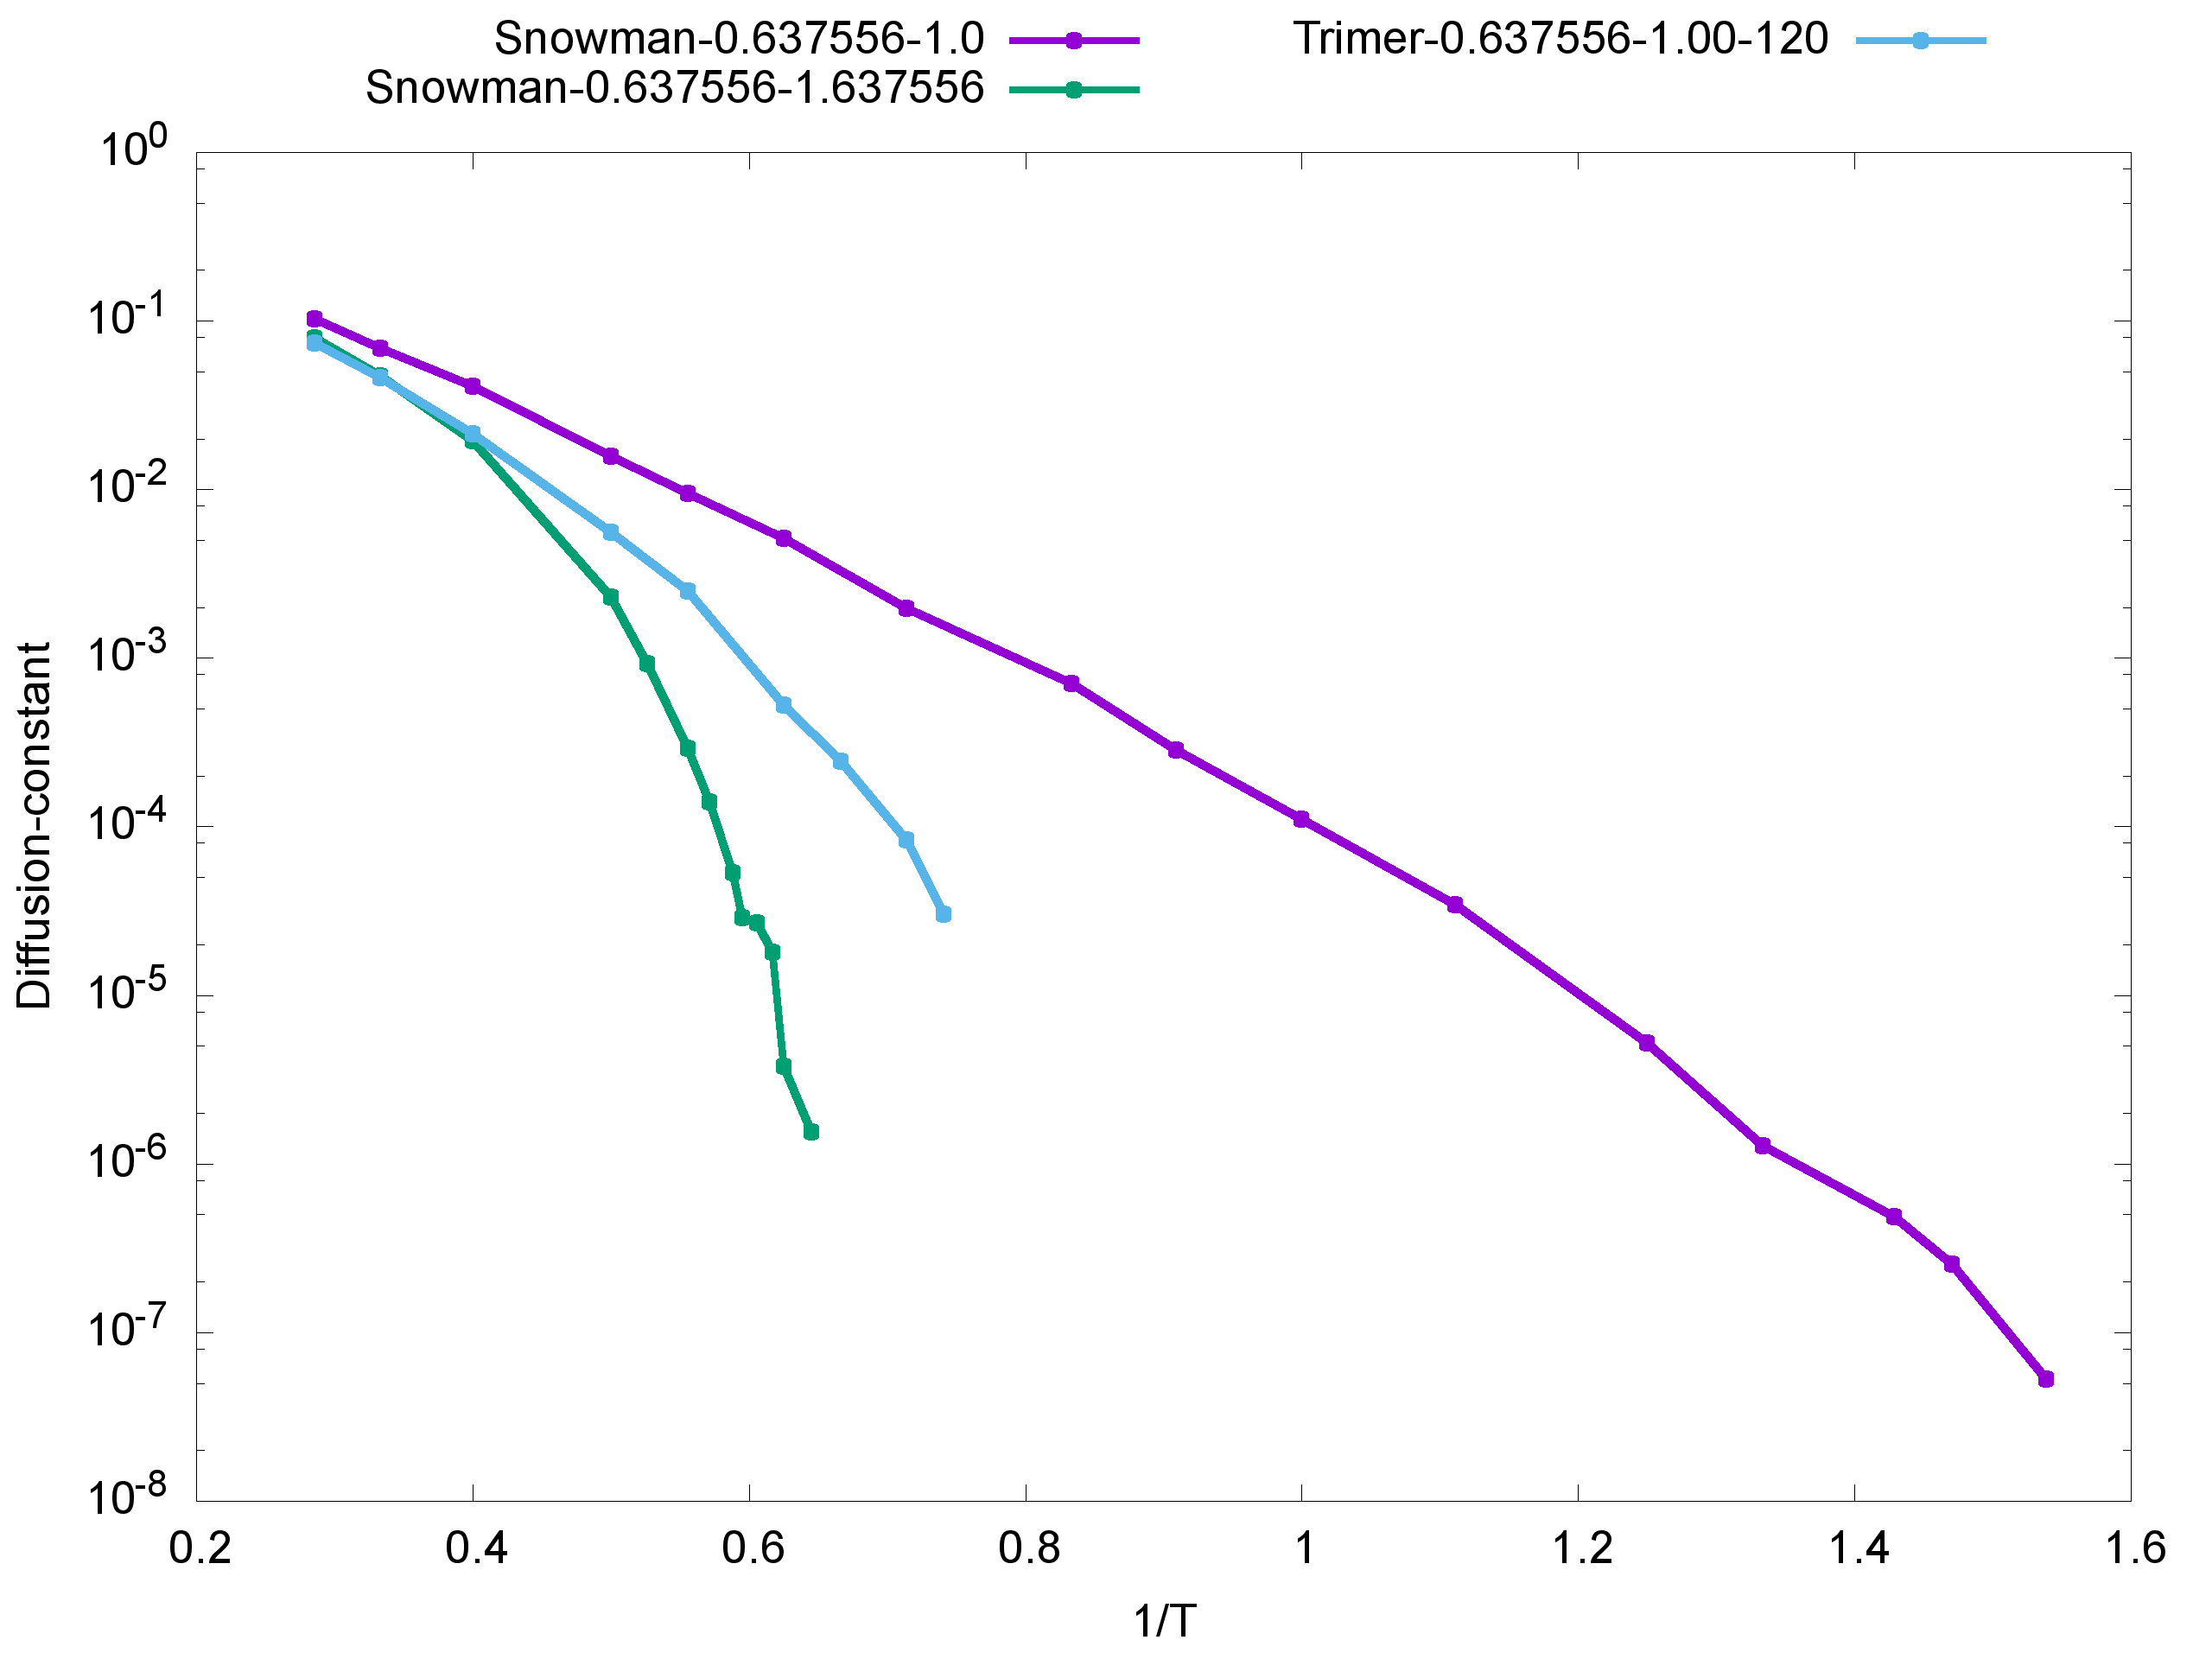
\includegraphics[width=\textwidth]{Diffusion-constant}
        \caption{Diffusion constant for all molecules}
        \label{fig:diffusion constant}
    \end{subfigure}
    \begin{subfigure}{0.5\linewidth}
        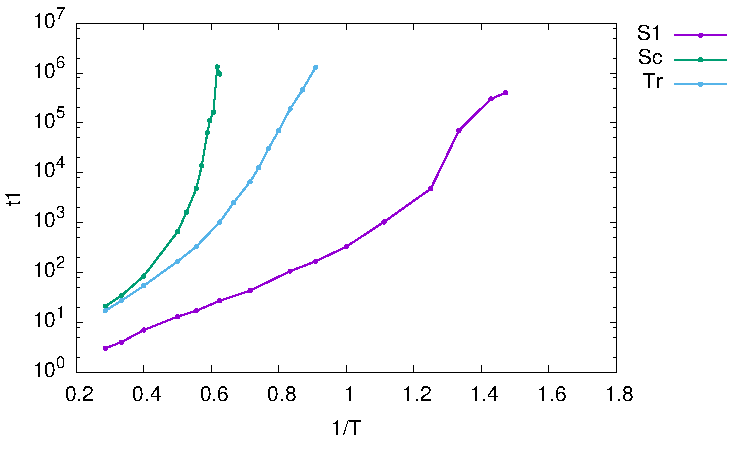
\includegraphics[width=\textwidth]{t1}
        \caption{Rotational relaxation time t1}
        \label{fig:tau1}
    \end{subfigure}
    \begin{subfigure}{0.5\textwidth}
        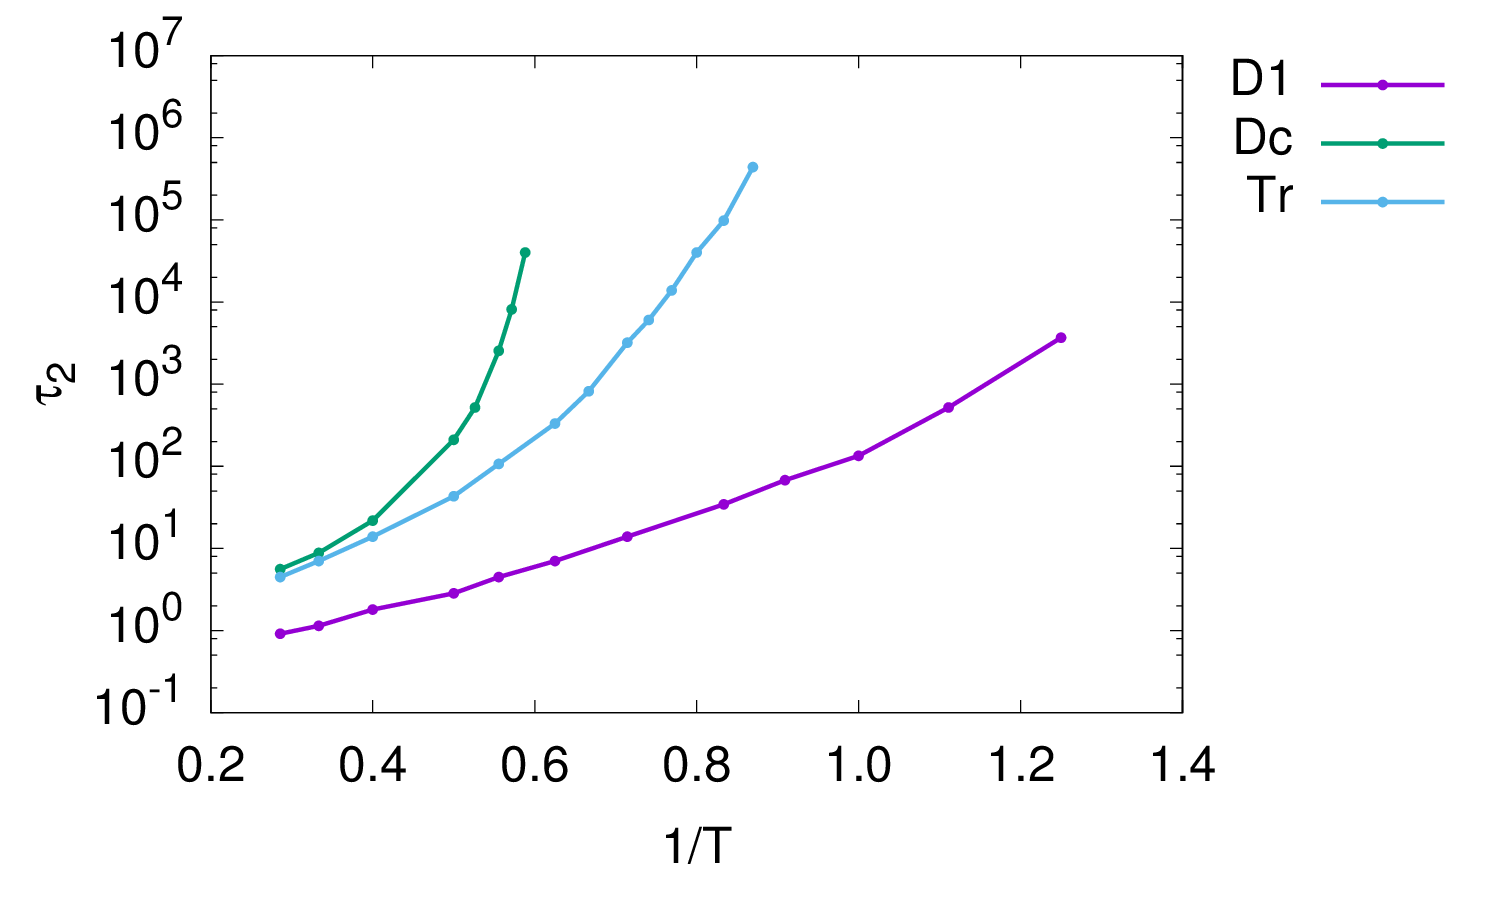
\includegraphics[width=\textwidth]{t2}
        \caption{Rotational relaxation time t2}
        \label{fig:tau2}
    \end{subfigure}
    \begin{subfigure}{0.5\textwidth}
        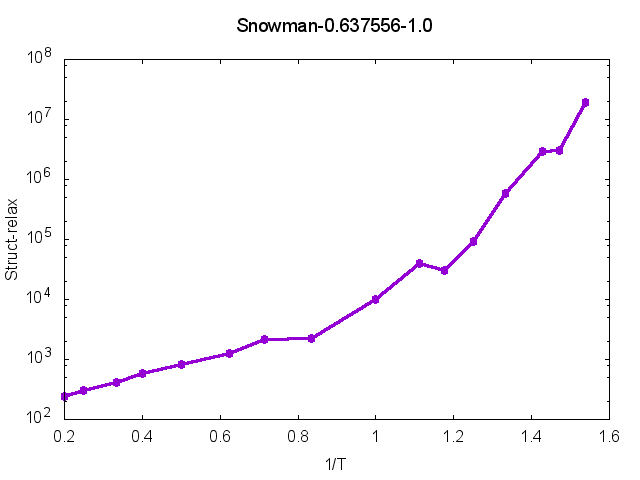
\includegraphics[width=\textwidth]{struct-relax}
        \caption{Structural relaxation times}
        \label{fig:struct relax}
    \end{subfigure}
    \caption{Comparison of dynamics quantities}
    \label{fig:dynamic comparison}
\end{figure}

From \textfigref{diffusion constat} we can see that as the size of the concavity increases from \sone, through \scon to \tri the fragility increases. This suggests that molecular shape is one of the features responsible for the fragility and by extension the formation of the glassy phase.
